\documentclass[tikz,border=12pt]{standalone}
\usepackage[T1]{fontenc}
\usepackage{mathpazo}
\usepackage{amsmath,amssymb}
\usetikzlibrary{arrows.meta, positioning, calc}

\definecolor{stblue}{HTML}{7B97AD}
\definecolor{rwgold}{HTML}{B8995E}
\definecolor{sage}{HTML}{7A9A7E}
\definecolor{dkbrown}{HTML}{3D3530}
\definecolor{wmgray}{HTML}{7B7067}
\definecolor{cream}{HTML}{F9F6F0}
\definecolor{border}{HTML}{D4C9B8}
\definecolor{terracotta}{HTML}{C47A6A}

\begin{document}
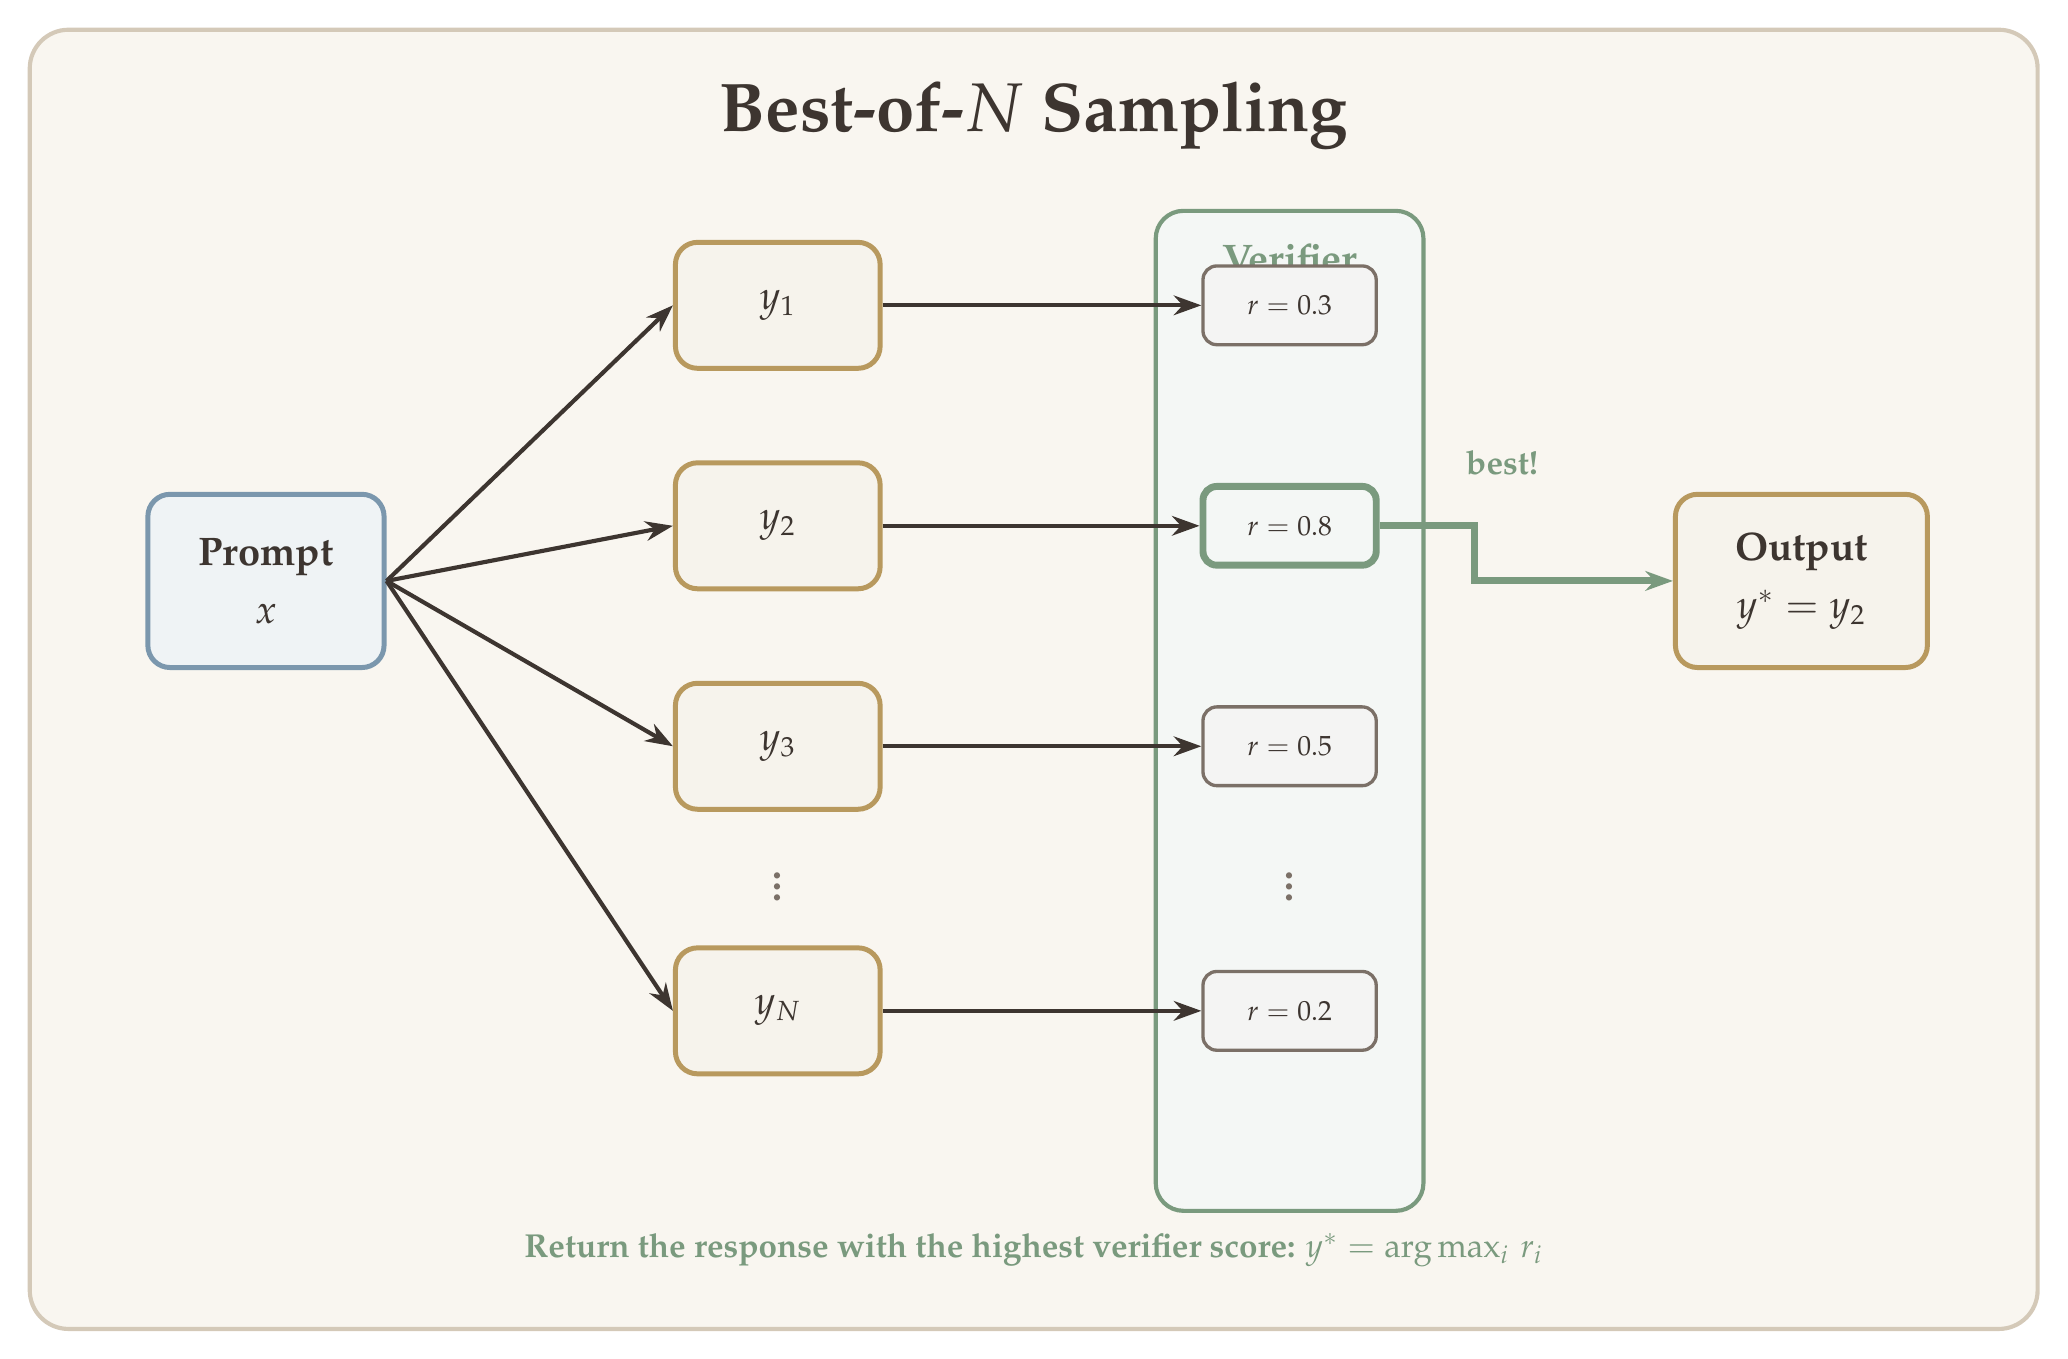
\begin{tikzpicture}[
  >={Stealth[length=3.5mm, width=2.5mm]},
  rbox/.style 2 args={
    draw=#1, line width=1.8pt, fill=#1!12, rounded corners=8pt,
    minimum width=26mm, minimum height=16mm, font=\Large,
    text=dkbrown, align=center, inner sep=5pt
  },
  scorebox/.style 2 args={
    draw=#1, line width=1.2pt, fill=#1!8, rounded corners=5pt,
    minimum width=22mm, minimum height=10mm, font=\normalsize,
    text=dkbrown, align=center, inner sep=3pt
  },
  arr/.style={->, line width=2pt, dkbrown},
  fanarr/.style={->, line width=1.5pt, dkbrown},
  note/.style={font=\normalsize, text=wmgray, align=center},
]

% Background
\fill[cream, rounded corners=14pt] (-1.5,-2) rectangle (24,14.5);
\draw[border, rounded corners=14pt, line width=1.5pt] (-1.5,-2) rectangle (24,14.5);

% Title
\node[font=\Huge\bfseries, text=dkbrown] at (11.25,13.4)
  {Best-of-$N$ Sampling};

% Prompt box (left)
\node[rbox={stblue}{}, minimum width=30mm, minimum height=22mm] (prompt) at (1.5,7.5)
  {\textbf{Prompt}\\[3pt] $x$};

% Response boxes (fan-out)
\def\respY{11}
\def\respSpacing{2.8}

\node[rbox={rwgold}{}] (r1) at (8, \respY)
  {\textbf{$y_1$}};
\node[rbox={rwgold}{}] (r2) at (8, \respY - \respSpacing*1)
  {\textbf{$y_2$}};
\node[rbox={rwgold}{}] (r3) at (8, \respY - \respSpacing*2)
  {\textbf{$y_3$}};
\node[font=\Large\bfseries, text=wmgray] at (8, \respY - \respSpacing*2.6)
  {$\vdots$};
\node[rbox={rwgold}{}] (rN) at (8, \respY - \respSpacing*3.2)
  {\textbf{$y_N$}};

% Fan-out arrows from prompt
\draw[fanarr] (prompt.east) -- (r1.west);
\draw[fanarr] (prompt.east) -- (r2.west);
\draw[fanarr] (prompt.east) -- (r3.west);
\draw[fanarr] (prompt.east) -- (rN.west);

% Verifier region
\fill[sage!8, rounded corners=10pt] (12.8, -0.5) rectangle (16.2, 12.2);
\draw[sage, line width=1.5pt, rounded corners=10pt] (12.8, -0.5) rectangle (16.2, 12.2);
\node[font=\Large\bfseries, text=sage] at (14.5, 11.6)
  {Verifier};

% Score boxes inside verifier
\node[scorebox={wmgray}{}] (s1) at (14.5, \respY)
  {$r = 0.3$};
\node[scorebox={sage}{}, draw=sage, line width=2.5pt] (s2) at (14.5, \respY - \respSpacing*1)
  {\textbf{$r = 0.8$}};
\node[scorebox={wmgray}{}] (s3) at (14.5, \respY - \respSpacing*2)
  {$r = 0.5$};
\node[font=\Large\bfseries, text=wmgray] at (14.5, \respY - \respSpacing*2.6)
  {$\vdots$};
\node[scorebox={wmgray}{}] (sN) at (14.5, \respY - \respSpacing*3.2)
  {$r = 0.2$};

% Arrows from responses to scores
\draw[fanarr] (r1.east) -- (s1.west);
\draw[fanarr] (r2.east) -- (s2.west);
\draw[fanarr] (r3.east) -- (s3.west);
\draw[fanarr] (rN.east) -- (sN.west);

% "best!" label for y2
\node[font=\large\bfseries, text=sage] at (17.2, \respY - \respSpacing*1 + 0.8)
  {best!};

% Output box
\node[rbox={rwgold}{}, minimum width=32mm, minimum height=22mm] (output) at (21, 7.5)
  {\textbf{Output}\\[3pt] $y^* = y_2$};

% Arrow from best score to output
\draw[arr, sage, line width=2.5pt] (s2.east) -- ++(1.2,0) |- (output.west);

% Bottom annotation
\node[font=\large\bfseries, text=sage] at (11.25,-1)
  {Return the response with the highest verifier score:
   $y^* = \arg\max_i\, r_i$};

\end{tikzpicture}
\end{document}
